\documentclass{article}

% to avoid loading the natbib package, add option nonatbib:
% \usepackage[nonatbib]{style}

\usepackage[final]{style}

\usepackage[utf8]{inputenc} % allow utf-8 input
\usepackage[T1]{fontenc}    % use 8-bit T1 fonts
\usepackage{hyperref}       % hyperlinks
\usepackage{url}            % simple URL typesetting
\usepackage{booktabs}       % professional-quality tables
\usepackage{amsfonts}       % blackboard math symbols
\usepackage{nicefrac}       % compact symbols for 1/2, etc.
\usepackage{microtype}      % microtypography
\usepackage{amsmath}
\usepackage{verbatim}
\usepackage{graphicx}
\usepackage{caption}

\title{Lecture 10: Semantic Segmentation and Clustering}

\author{
  \textbf{Vineet Kosaraju, Davy Ragland, Adrien Truong, Effie Nehoran, Maneekwan Toyungyernsub} \\
  Department of Computer Science\\
  Stanford University\\
  Stanford, CA 94305 \\
  \texttt{\{vineetk, dragland, aqtruong, effie, maneekwt\}@cs.stanford.edu} \\
}

\begin{document}

\maketitle

\section{Clustering and Segmentation}
Image segmentation is a task in computer vision; it aims to identify groups of pixels and image regions that are similar and belong together. Different similarity measures can be used for grouping pixels; this includes texture and color features. An instance of image segmentation is illustrated below. In Figure 1, the objective is to group all the pixels that make up the tiger, the grass, the sky, and the sand. The resulting segmentation can be observed in Figure 2.

\begin{figure}[!htb]
   \begin{minipage}{0.48\textwidth}
     \centering
     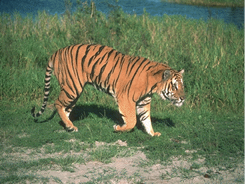
\includegraphics[width=.7\linewidth]{tiger.png}
     \caption{Input image. Source: lecture 12, slide 4}
   \end{minipage}\hfill
   \begin {minipage}{0.48\textwidth}
     \centering
     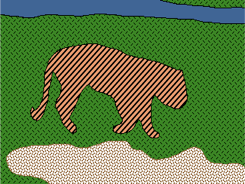
\includegraphics[width=.7\linewidth]{tiger-segmented.png}
     \caption{Output segmentation. Source: lecture 12, slide 4}
   \end{minipage}
\end{figure}

Other examples of image segmentation include grouping video frames into shots and separating an image's foreground and background. By identifying the groups of pixels that belong together, an image can be broken down into distinct objects. In addition to its immediate use for object recognition, this can also allow for greater efficiency in any further processing.


\section{Gestalt School and Factors}
Many computer vision algorithms draw from the areas outside of computer science, and image segmentation is no different. Computer vision researchers drew inspiration from the field of psychology, specifically the Gestalt Theory of Visual Perception. At a very high level, this theory states that "the whole is greater than the sum of its parts." The relationships between parts can yield new properties and features. This theory defines Gestalt factors, properties that can define groups in images. Below are examples of such factors.

\begin{center}
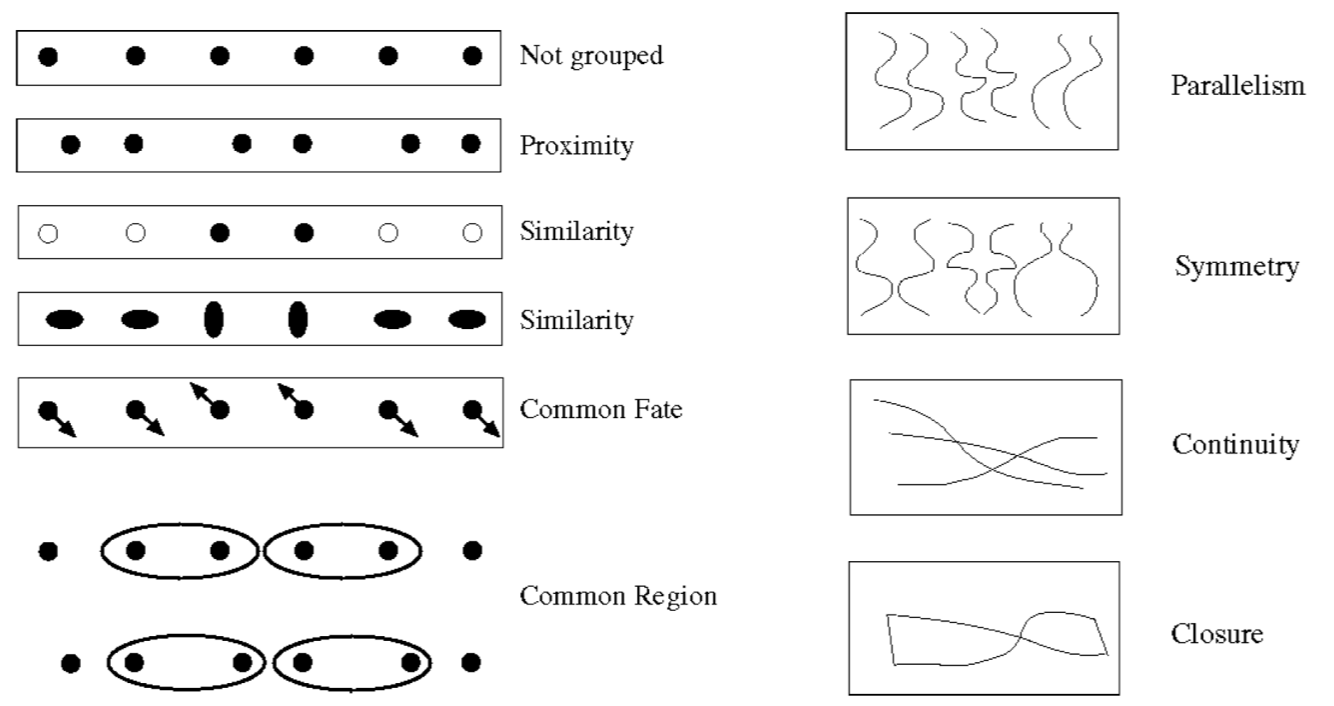
\includegraphics[width=0.8\textwidth]{gestalt-factors.png}
\captionof{figure}{Examples of gestalt factors. Source: Forsyth \& Ponce \cite{forsyth2011computer}}
\end{center}

Here is an example of an other factor; while Figure 4 does not appear to have meaningful visual content, the addition of the overlaying gray lines  (Figure 5) on the same image provides visual cues as to the pixel groupings and image content.

\begin{figure}[!htb]
	\begin{minipage}{0.48\textwidth}
		\centering
		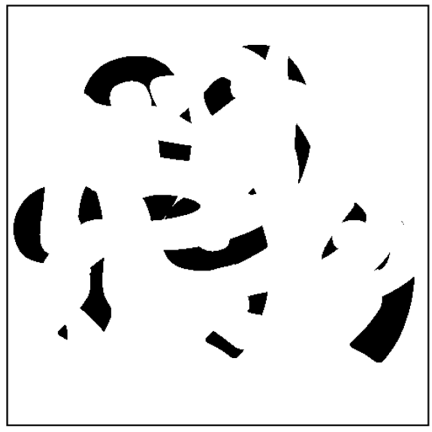
\includegraphics[width=.7\linewidth]{continuity-occlusion.png}
		\caption{Source: Forsyth \& Ponce \cite{forsyth2011computer}}
	\end{minipage}\hfill
	\begin {minipage}{0.48\textwidth}
	\centering
	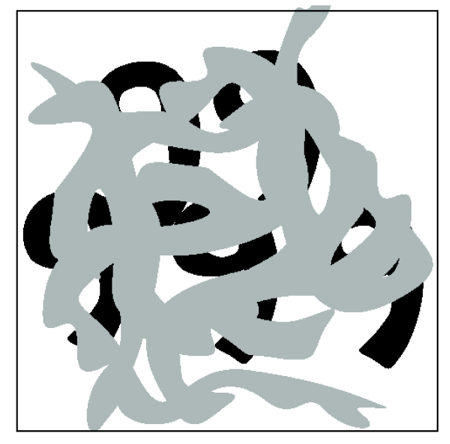
\includegraphics[width=.7\linewidth]{continuity-occlusion-2.png}
	\caption{Source: Forsyth \& Ponce \cite{forsyth2011computer}}
\end{minipage}
\end{figure}


We can now more clearly see that the image is a few 9's occluded by the gray lines. This is an example of a continuity through occlusion cue. The gray lines give us a cue that the black pixels are not separate and should in fact be grouped together. By grouping the black pixels together and not perceiving them as separate objects, our brain is able to recognize that this picture contains a few digits.

Below is another example:
\begin{center}
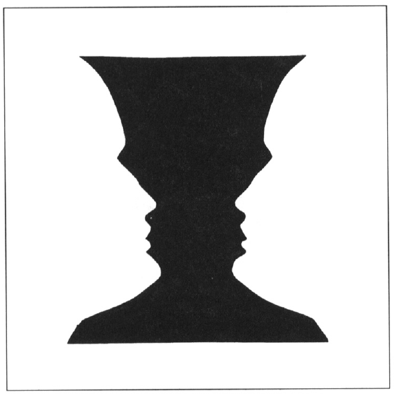
\includegraphics[width=0.5\textwidth]{figure-ground.png}
\captionof{figure}{Source: Forsyth \& Ponce \cite{forsyth2011computer}}
\end{center}

What do you see? Do you see a cup or do you see the side of 2 heads facing each other? Either option is correct, depending on your perspective. This variation in perception is due to what we identify as the foreground and the background. If we identify the black pixels as the foreground, we see a cup. But, if we identify the white pixels as the foreground, we see 2 faces.

This is an overview of some of the factors that affect human's perception of pixel/image region grouping within visual data. One thing to note, however, is that while these factors may be intuitive, it's hard to translate these factors into working algorithms.

How do we perform image segmentation? What algorithms do we use? One way to think about segmentation is clustering. We have a few pixels and we want to assign each to a cluster. In the following sections, different methods of clustering will be detailed.

\section{Agglomerative Clustering}

Clustering is an unsupervised learning technique where several data points, $x_1, ..., x_n$, each of which are in $R^D$, are grouped together into clusters without knowing the correct label/cluster. \textbf{Agglomerative clustering} is one of the commonly used techniques for clustering.

The general idea behind agglomerative clustering is to look at similarities between points to decide how these points should be grouped in a sensible manner. Before we discuss the details of the algorithm, we must first decide how we determine similarity.

\subsection{Distance Measures}

We measure the similarity between objects by determining the distance between them: the smaller the distance, the higher the degree of similarity. There are several possible distance functions, but it is hard to determine what makes a good distance metric, so usually the focus is placed on standard, well-researched distance metrics such as the two detailed below.

\subsubsection{Euclidean Distance}

One common measure of similarity is the Euclidean distance; it measures the distances between two data points, $x$ and $x'$ by taking into account the angle and the magnitude. We can write the Euclidean distance as the following:

\begin{equation}
	sim(x, x') = x^T x'
\end{equation}

This distance measure does not normalize the vectors, so their magnitude is factored into the similarity calculations.

\subsubsection{Cosine Similarity Measure}

Another common solution is the Cosine similarity measure; it only accounts for the angle between two data points, $x$ and $x'$. Note that \textbf{unlike the Euclidean distance}, the cosine measure only represents \textit{similarity}, not \textit{distance}. This means that the similarity between a data point $x$, and itself, equals 1. As its name implies, this measure relies on the cosine between the two points, as found by:

\begin{equation}
	sim(x, x') = cos(\theta)
\end{equation}
\begin{equation}
	= \frac{x^T x'}{||x|| \cdot ||x'||}
\end{equation}
\begin{equation}
	= \frac{x^T x'}{ \sqrt{x^T x} \sqrt{{x'}^T x'} }
\end{equation}

The division by the magnitudes of the vectors results in the normalization of the distance metric, and it ensure that the measure is only dependent on the angle between the objects.

\subsection{Desirable Clustering Properties}

Now that the potential distance metrics are defined, the next step is to choose a clustering technique. There are various properties of clustering methods that we might want to consider when choosing specific techniques:

\begin{enumerate}
	\item \textbf{Scalable} - in terms of compute power \& memory
	\item \textbf{Different data types} - algorithm should support arbitrary data being in $R^d$ for all $d$
	\item \textbf{Input parameters} - The parameter tuning for the algorithm should not be difficult. The algorithm is more useful if it does not heavily rely on our accurate understanding of the data.
	\item \textbf{Interpretable} - we should be able to interpret the results.
	\item \textbf{Constraints} - The algorithm should effectively use the predefined constraints (e.g., we know two points should be in the same cluster, or they shouldn't belong together).
\end{enumerate}

The following sections cover the implementation of the  agglomerative clustering and its benefits and drawbacks.

\subsection{Agglomerative Clustering Implementation}

The agglomerative clustering calculates the similarities among data points by grouping closer points together. The newly created groups can further be merged to other groups that are close to them; this iterative process results in the generation of bigger groups until there only remains one group. This creates a hierarchy, best viewed as a \textbf{dendrogram}.

We can visualize this in the following diagram, which shows data points and the results of an agglomerative clustering algorithm.

\begin{minipage}{\linewidth}
\begin{center}
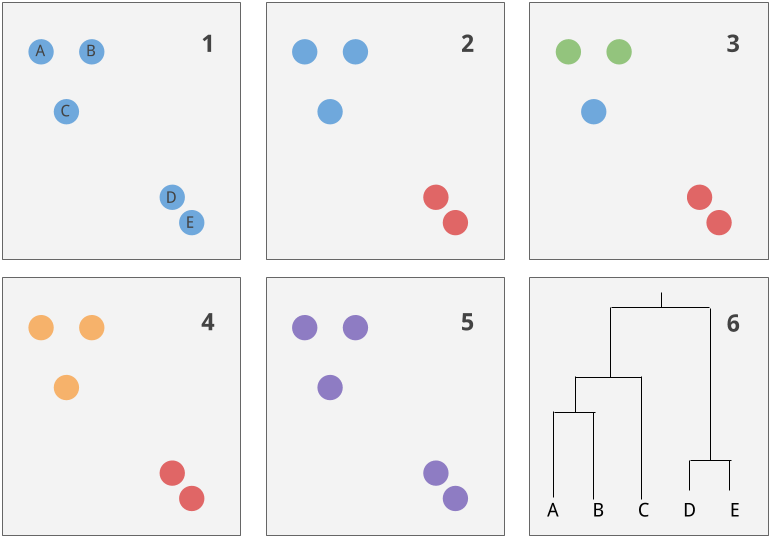
\includegraphics[width=0.70\textwidth]{dendrogram2.png}
\captionof{figure}{Agglomerative clustering on sample input, and resulting dendrogram}
\end{center}
\end{minipage}

The first picture shows all the data points, and pictures 2 to 5 show various steps in the clustering algorithm. Step 2 groups the two red points together; step 3 groups the two green points together; step 4 groups the previous green group and the nearby blue point into a new orange group; and step 5 groups all the points together into one large group. This creates the dendrogram in picture 6.

\subsubsection{Algorithm}

Our general algorithm is based on our intuition and has four main steps:

\begin{enumerate}
	\item Initialize each point as its own cluster
	\item Find the most similar pair of clusters
	\item Merge the similar pair of clusters into a \textit{parent} cluster
	\item Repeat steps 2 \& 3 until we have only 1 cluster.
\end{enumerate}

\subsubsection{Questions}

Although agglomerative clustering is a powerful technique, various factors should be taken into consideration when implementing it. For instance:

\begin{enumerate}
	\item \textit{How do we define similarity between clusters? How do we measure the distance between two clusters?}
	
	We can measure the distance between two clusters in a variety of different ways including the average distance between points, the minimum distance between points in the clusters, the distance between the means of each cluster, and the maximum distance between points in the clusters. The method used for measuring the distance between clusters can highly affect the results.
	
	\item \textit{How many clusters do we chose?}
	
	When we create the dendrogram, we can decide how many clusters we want based on a distance threshold. Alternatively, we can cut the dendrogram horizontally at its different levels to create as many clusters as we want.
	
\end{enumerate}

\subsection{Different measures of nearest clusters}
There are three main models we can use to determine the distance between cluster points as we segment our dataset: single, complete, and average.

\begin{enumerate}
	\item Single link:\\
	Distance is calculated with the formula:
	\begin{equation}
	    d(C_i,C_j) = min_{x \in C_i,x' \in C_j}d(x,x')
    \end{equation}
    With single linkage, we cluster by utilizing the minimum distance between points in the two clusters.\\
    This is also known as a minimum spanning tree.\\
    We can stop clustering once we pass a threshold for the acceptable distance between clusters.\\
    This algorithm tends to produces long, skinny clusters (since it is very easy to link far away points to be in the same cluster as we only care about the point in that cluster with the minimum distance).
    \begin{center}
        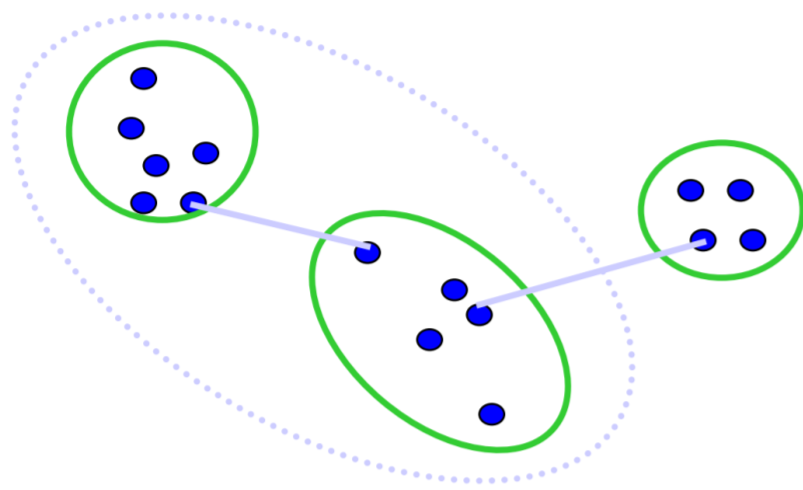
\includegraphics[width=0.70\textwidth]{single.png}
        \captionof{figure}{Image segmentation example using single link measurement of nearest clusters. Source: lecture 12, slide 46}
    \end{center}

	\item Complete link:\\
	Distance is calculated with the formula:
	\begin{equation}
	    d(C_i,C_j) = max_{x \in C_i,x' \in C_j}d(x,x')
    \end{equation}
    With complete linkage, we cluster by utilizing the maximum distance between points in the two clusters.\\
    This algorithm tends to produces compact and tight clusters of roughly equal diameter (since it favors having all the points close together).
    \begin{center}
        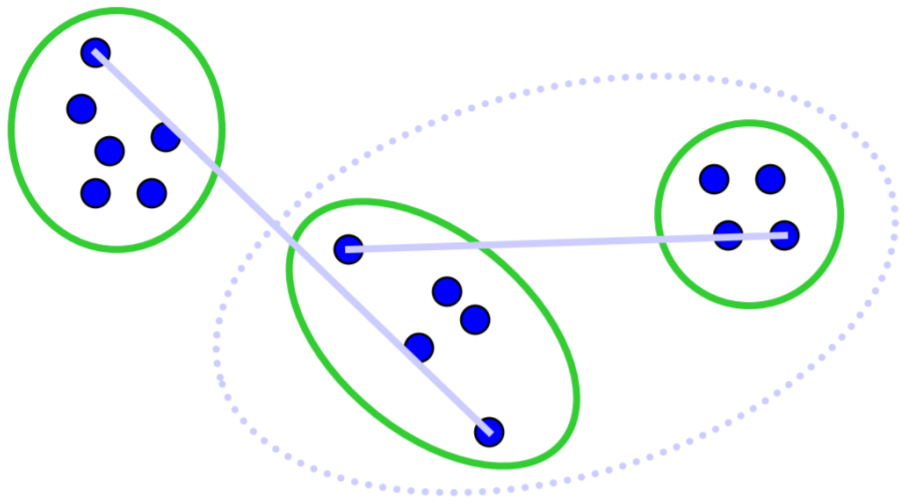
\includegraphics[width=0.70\textwidth]{complete.png}
        \captionof{figure}{Image segmentation example using complete link measurement of nearest clusters. Source: lecture 12, slide 47}
    \end{center}

	\item Average link:\\
	Distance is calculated with the formula:
	\begin{equation}
	    d(C_i,C_j) = \frac{\sum x \in C_i,x' \in C_j d(x,x')}{|C_i|\cdot |C_j|}
    \end{equation}
    With average linkage, we cluster by utilizing the average distance between points in the two clusters.\\
    This model is robust against noise because the distance does not depend on single pair of points unlike single links and complete links, where points can be affected by artifacts in the data.
    \begin{center}
        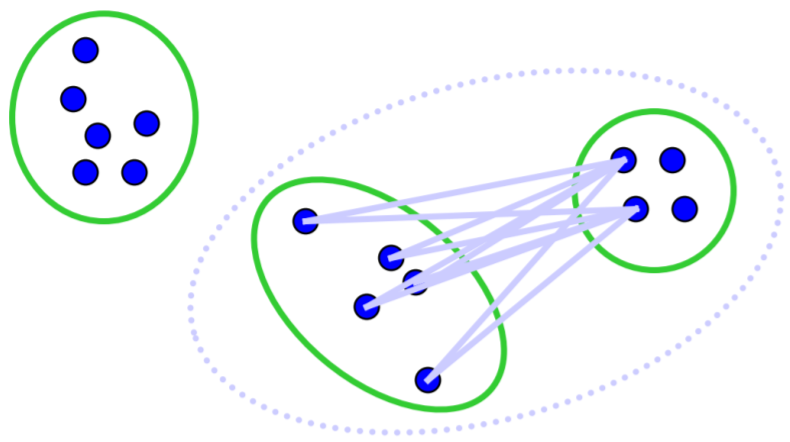
\includegraphics[width=0.70\textwidth]{average.png}
        \captionof{figure}{Image segmentation example using average link measurement of nearest clusters. Source: lecture 12, slide 48}
    \end{center}
\end{enumerate}

\subsection{Agglomerative clustering conclusions}

The positive characteristics of agglomerative clustering:
\begin{enumerate}
	\item Simple to implement and apply
	\item Cluster shape adapts to dataset
	\item Results in a hierarchy of clusters
	\item No need to specify number of clusters at initialization
\end{enumerate}

In terms of its negative characteristics:
\begin{enumerate}
	\item Can return imbalanced clusters
	\item Threshold value for number of clusters must be specified
	\item Does not scale well with a runtime of $O(n^3)$
	\item Greedy merging can get stuck at local minima
\end{enumerate}

\section{K-Means Clustering}
Another algorithm is k-means clustering. It identifies a fixed number of cluster "centers" as representatives of their clusters, and labels each point according to the center it is closest to. A major difference between k-means and agglomerative clustering is that k-means requires the input of a target number of clusters to run the algorithm.
\subsection{Image Segmentation Example}
At the top left of figure 11, we have an image with three distinct color regions, so segmenting the image using color intensity can be achieved by assigning each color intensity, shown on the top right, to a different cluster. In the bottom left image, however, the image is cluttered with noise. To segment the image, we can use k-means.

\begin{minipage}{\linewidth}
\begin{center}
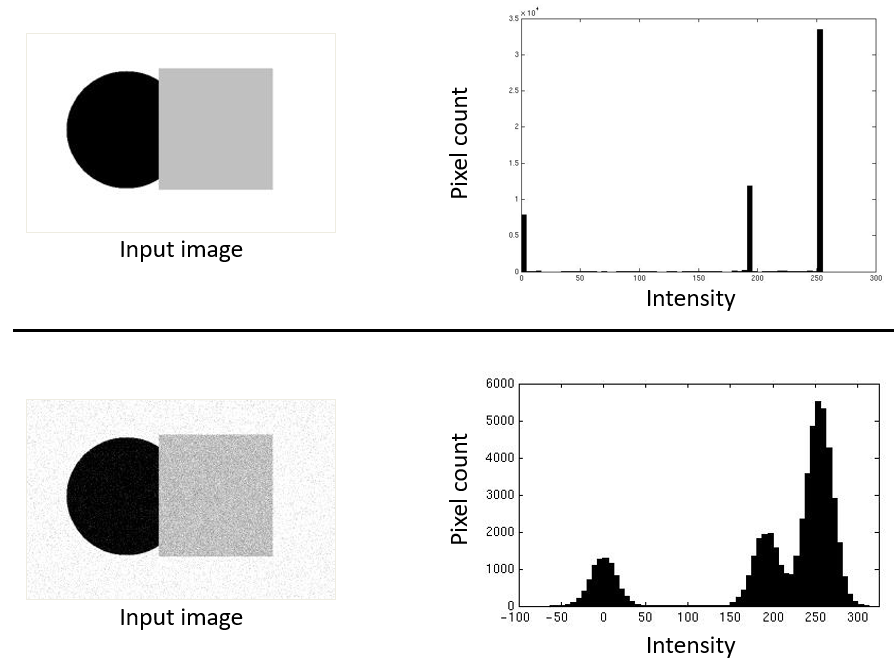
\includegraphics[width=0.70\textwidth]{k-means-example.png}
\captionof{figure}{Image segmentation example using k-means. The picture on the top left has three distinct colors, but the bottom picture has Gaussian noise. Source: lecture 11, slide 8, slide credit: Kristen Grauman}
\end{center}
\end{minipage}

Using k-means, the objective here is to identify three cluster centers as the representative intensities, and label each pixel according to its closest center. The best cluster centers are those that minimize Sum of Square Distance between all points and their nearest cluster center $c_i$:
\begin{equation}
SSD = \sum_{i \in \textrm{clusters}}\sum_{x \in \textrm{cluster}_i}(x-c_i)^2
\end{equation}

When we are using k-means to summarize a dataset, the goal is to minimize the variance in the data points that are assigned to each cluster. We would like to preserve as much information as possible given a certain number of clusters. This is demonstrated by the equation below.
\begin{minipage}{\linewidth}
\begin{center}
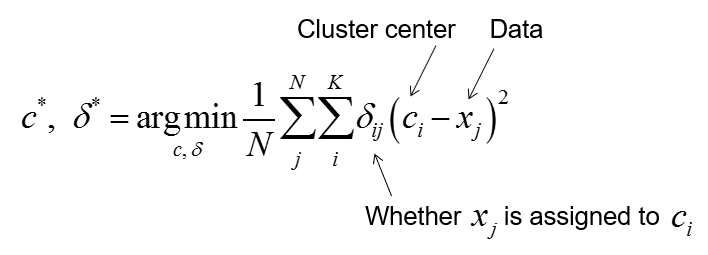
\includegraphics[width=0.70\textwidth]{clustering_for_summarization.png}
\captionof{figure}{Clustering for summarization. Source: lecture 11, slide 11}
\end{center}
\end{minipage}

\subsection{Algorithm}
Finding the cluster centers and group memberships of points can be thought of as a "chicken and egg" problem. If we knew the cluster centers, we could allocate points to groups by assigning each point to the closest center. On the other hand, if we knew the group memberships, we could find the centers by computing the mean of each group. Therefore, we alternate between the tasks.

In order to find the centers and group memberships, we start by initializing k cluster centers, usually by assigning them randomly. We then run through an iterative process that computes group memberships and cluster centers for a certain number of iterations or until the values of the cluster centers converge. The process is outlined below:

\begin{enumerate}
    \item Initialize cluster centers $c_1, ... , c_K$. Usually, these centers are randomly chosen data points.
    \item Assign each point in the dataset to the closest center. As in agglomerative clustering, we can use the Euclidean distance or the cosine distance measure to compute the distance to each center.
    \item Update the cluster centers to be the mean of the points in the cluster's group.
    \item Repeat Steps 2-3 until the value of the cluster centers stops changing or the algorithm has reached the maximum number of iterations.
\end{enumerate}

\begin{minipage}{\linewidth}
\begin{center}
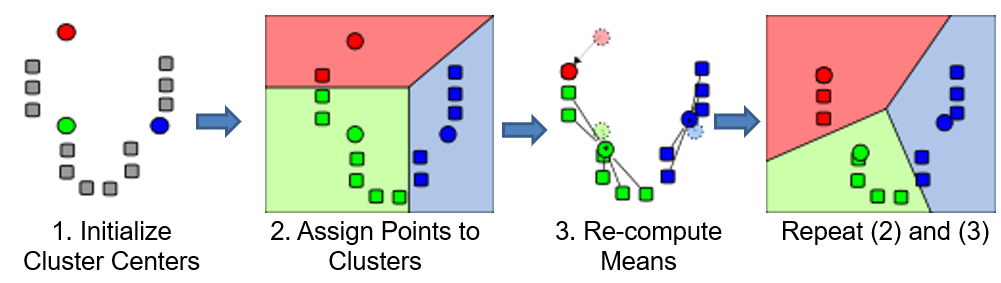
\includegraphics[width=0.70\textwidth]{k-means-algorithm.png}
\captionof{figure}{Visualization of k-means clustering. Source: lecture 11, slide 15}
\end{center}
\end{minipage}

\subsection{Output}
Each time it is run, k-means converges to a local minimum solution. Additionally, since the centers are initialized randomly, each run of the algorithm may return a different result. Therefore, initializing multiple runs of k-means and then choosing the most representative clustering yields the best results. The best clustering can be measured by minimizing the sum of the square distances to the centers or the variance of each cluster. K-means works best with spherical data.

\subsection{Segmentation as Clustering}
As with the example in section 4.1, clustering can be used to segment an image. While color intensity alone can be effective in situations like Figure 11, others such as Figure 14 may require us to define a feature space, in which we choose which features of pixels should be used as input to the clustering. In other words, the choice of feature space directly affects the calculation of the similarity measure between data points; the creative choice of feature space enables us to "represent" the data points in a way that clusters are more easily distinguishable from each other.

\begin{minipage}{\linewidth}
\begin{center}
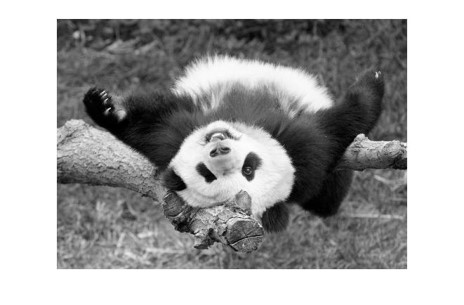
\includegraphics[width=0.70\textwidth]{panda.jpg}
\captionof{figure}{Image of a panda. Source: lecture 11, slide 19}
\end{center}
\end{minipage}

In addition to pixel intensity, examples of pixel groupings using an image feature space include RGB color similarities, texture similarities, and pixel positions. Clustering based on color similarities can be modeled using separate features for red, green, and blue. Texture can be measured by the similarities of pixels after applying specific filters. Position features include the coordinates of pixels within an image. Both intensity and position can be used together to group pixels based on similarity and proximity.

\subsection{K-Means++}
K-means method is appealing due to its speed and simplicity but not its accuracy. By augmentation with a variant on choosing the initial seeds for the k-means clustering problems, arbitrarily bad clusterings that are sometimes a result of k-means clustering may be avoided. The algorithm for choosing the initial seeds for k-means++ is outlined as following:
\begin{enumerate}
    \item Randomly choose a starting center from the data points
    \item Compute a distance $D(X)$, which is a distance between each data point $x$ to the center that has been chosen. By using a weighted probability distribution, a new data point is chosen as a new center based on a probability that is proportional to $D(x)^2$
    \item Repeat the previous step until $k$ centers have been chosen and then proceed with the usual k-means clustering process as the initial seeds have been selected
\end{enumerate}
It has been shown that k-means++ is Olog(K) competitive.

\subsection{Evaluation of clusters}
The clustering results can be evaluated in various ways. For example, there is an $internal$ evaluation measure, which involves giving a single quality score the results. $External$ evaluation, on the other hand, compares the clustering results to an existing true classification. More qualitatively, we can evaluate the results of clustering based on its $generative$ measure: how well is the reconstruction of points from the clusters or is the center of the cluster a good representation of the data. Another evaluation method is a $discriminative$ method where we evaluate how well clusters correspond to the labels. We check if the clusters are able to separate things that should be separated. This measure can only be worked with supervised learning as there are no labels associated with unsupervised learning. 

\subsection{Pros \& Cons}
There are advantages and disadvantages associated with k-means clustering technique:


\textbf{Pros}
\begin{enumerate}
\item Simple and easy to implement
\item Fast for low-dimensional data
\item Good representation of the data (cluster centers minimize the conditional variance)
\end{enumerate}
\textbf{Cons}
\begin{enumerate}
\item Doesn't identify outliers
\item Need to specify $k$ value, which is unknown 
\item Cannot handle non-globular data of different sizes and densities
\item Restricted to data which has the notion of a center 
\item Converge to a local minimum of the objective function instead and is not guaranteed to converge to the global minimum of the objective function
\end{enumerate}
In order to choose the number of clusters or the $k$ value, the objective function can be plotted against different $k$ values. The abrupt change in the objective function at a certain $k$ value is suggestive of that specific number of clusters in the data. This technique is called "knee-finding" or "elbow-finding"

\section{Mean-shift Clustering}
Mean-shift clustering is yet another clustering algorithm. At its essence, mean-shift clustering is about finding the densest areas in our feature space. This algorithm has four main steps:
\begin{enumerate}
    \item Initialize random seed, and window W
    \item Calculate center of gravity (the "mean) of W: $\displaystyle \sum_{x \in W} xH(x)$
    \item Shift the search window to the mean
    \item Repeat step 2 until convergence
\end{enumerate}
One way to mentally visualize this algorithm is to picture each data point as a marble. If each marble is attracted to areas of high density, all the marbles will eventually converge onto 1 or more centers.

We can also try to visualize the algorithm via this picture:
\begin{center}
\centering
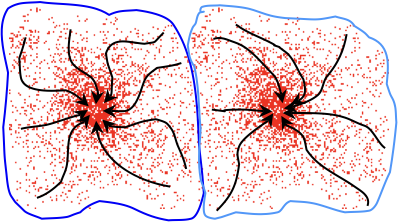
\includegraphics[width=0.5\textwidth]{mean-shift.png}
\captionof{figure}{Results of mean-shift clustering.\\Source: Y. Ukrainitz \& B. Sarel}
\end{center}
In this picture, we see the algorithm will generate 2 clusters. All the data points on the left converge onto one center and all the data points on the right converge onto a different center.
\\~\\
To learn more about mean-shift clustering please refer to the next set of notes.

% References
\small
\bibliographystyle{plain}
\bibliography{bibliography}

\end{document}